In the following pages, \Cref{sec:theory_actors_and_choices} introduces the model, including the actors, their choices, and the assumptions behind the model. \Cref{sec:theory_tradeoff} discusses the official's budget constraint. I argue that, holding a firm's profit constant, the official faces a trade-off between spillover and private benefits since offering either good cuts into the profit of the firm. \Cref{sec:theory_budget_constraint_size} and \Cref{sec:theory_budget_constraint_slope_and_intercept} examine the parameters that change the location and the slope of the budget constraint. \Cref{sec:theory_indifference_curve} shows how the official's time horizon changes the shape of his indifference curve. Together, the official's budget constraint and indifference curve regarding spillover and private benefits determine his choice over this two-good bundle. Once equipped with this theoretical framework, we can derive testable hypotheses regarding the official's choice in the next part of the project. Finally, \Cref{sec:theory_literature_review} situates my model, showing how it conceptualizes corruption between the official and the foreign firm as \textit{symbiotic} rather than \textit{predatory} as the literature has always assumed.

\subsection{Actors and choices}
\label{sec:theory_actors_and_choices}

The model has one strategic actor: a government official. This official has control over a certain endowment (e.g. market access, cheap labor) that is attractive to foreign firms.\footnote{I define \textit{foreign firms} as firms with over 50\% ownership belonging to private foreign individuals, companies, or organizations. In these firms, we are certain that the foreign owner has the majority stake and is responsible for the firm's choice. This definition is common across business surveys and national laws, allowing us to collect a wide range of data.} Foreign firms who invest in the official's territory turn this endowment into profit via their productive activities. Firms then share the value added with the official in exchange for access to the endowment. 

Firms share the value added with the official in the form of a two-good bundle: 1) technological spillover and, 2) private benefits (to the official). \textit{Technological spillover} is the beneficial effects of foreign firms' technological knowledge on the productivity of domestic firms. The official cares about the technological spillover of FDI because it is a crucial ingredient in improving total factor productivity and generating long-term growth. Growth, in turn, brings electoral or career benefits. \textit{Private benefits} that firms offer to the official can come in many forms, both illegal (e.g. bribe, kickback) and legal (e.g. campaign finance contribution, informal network with foreign firms that leads to contracts for friends and families). I argue that offering either spillover or private benefits cuts into the firm's profit. Therefore, if the official wants more of one good from the firm it has to take less of the other. In other words, the official faces a trade-off between spillover and private benefits, and the essence of the dissertation is to determine how the official chooses the mix of this two-good bundle.

In this model, firms care about whether the official demands spillover or private benefits, but only because firms have heterogeneous abilities in offering these two goods. For example, if a firm belongs to an industry where production is divisible, it is easier and less expensive for the firm to sub-contract local firms and create spillover. On the other hand, if a firm comes from a country with little corruption, it may be less adept at working with the official. It will have to hire local agents, and thus finds it more expensive to offer the same amount of private benefits than firms that are more familiar with corrupt dealings. I model this firm's preference via two parameters: the ``price'' of spillover and the ``price'' of private benefits, which the official has to consider when he demands one of the two goods from the firm. By doing so, my model is able to incorporate firm's preference without introducing it as a strategic actor.

This model has two assumptions. First, offering spillover or private benefits only affects the firm's utility through its bottom line. If we believe that firms are unlikely to have moral (or other non-financial) incentives to bring spillover or to withhold bribe, then this assumption is reasonable. 

Second, I assume that the firm is satisfied as long as its retained profit remains above a reservation level. The firm will not invest if and only if the official's demand reduces its profit to below this level. This assumption is supported by the behavioral model of firms, in which firms are profit-satisficing instead of profit-maximizing \citep{Simon1959}. Granted, it is less defensible to build a model with one actor satisficing (the firm) while the other maximizing (the official). Therefore, in \Cref{sec:rd_tsl}, I will model both actors as utility maximizing, using two-sided logit (TSL) model to estimate their preferences. \citet{Logan1996a} has shown that TSL corresponds to the game-theoretic college admissions model, a many-to-one matching problem that is relevant to how countries and FDI firms find their match.


\subsection{The trade-off between spillover and private benefits}
\label{sec:theory_tradeoff}

To induce spillover, governments frequently impose on foreign firms conditions such as forming a joint venture or local content requirement. These conditions constrain firms' ability to optimally use their physical and management capital, reducing their profitability. Similarly, when firms are forced to offer private benefits to officials, they suffer from not only a upfront cost but also a uncertainty cost. This uncertainty stems from the frequent lack of transparency and the high degree of informality regarding these private benefits, making the process abstruse to foreign firms. For this reason, offering private benefits to the official increases firms' expenses and thus also reduces profitability. Given that 1) offering either spillover or private benefits cuts into the firm's profit, and that 2) the firm has to maintain a minimum amount of profit (akin to reservation wage) that justifies investing in the country, if a firm offers more private benefits to the official it will have to bring less technological spillover, and vice versa.

One may argue that some foreign firms voluntarily produce spillover---therefore, offering spillover and private benefits is not a trade-off. However, such cases are rare because foreign firms want to keep their technology proprietary and maintain their competitive advantage. Due to scale and sophistication, foreign firms also source from established international suppliers and only buy standard commodity goods from local suppliers at arms-length, which does not generate as much spillover as personal contact (e.g. training, quality assurance assistance, financing assistance). FDI firms voluntarily source from local suppliers only when the availability and the quality of local suppliers are not far from the international standard---however, in these cases there is less need and room for spillover to start with. Another scenario that leads to foreign firms voluntarily producing spillover is when they specifically target the local market. In this case, the qualilty requirement is not too stringent, the quantity not too large, and there is a need for rapid local customization. Unfortunately, in this case, market oriented FDI firms can displace local firms, which may lead to a net reduction in domestic firms' productivity \citep{Mody2004}.

In sum, given that offering either spillover or private benefits cuts into the firm's finite profit, the official can only have more of one good if he gives up some of the other. In other words, there is a trade-off between spillover and private benefits, and the official faces a budget constraint over this two-good bundle.

While FDI does bring other benefits, e.g. jobs and capital, my theory intentionally focuses on the trade-off between technological spillover and private benefits for both substantive and theoretical reasons. Substantively, technological spillover increases a country's total factor productivity (TFP), a key to sustained long-term economic growth in the face of diminishing returns to capital. While the literature has mainly focused on the quantity of FDI a country attracts, development agencies and governments have paid much attention to the quality of FDI, i.e. its technological spillover. 

Furthermore, the implication of a spillover-vs-private-benefit trade-off is very different from that of a spillover-vs-capital/job trade-off. In the later case, one can count on the official to shift towards attracting high spillover FDI as his country gradually grows and is in less immediate need of capital and job creation. The growth trajectory of a country is guaranteed to be positive in this scenario, fueled by FDI's capital injection in the earlier stage and sustained by FDI's technological transfer in the later stage. However, if the trade-off that the official considers is between spillover and private benefits as my project theorizes, then one cannot count on the official to take such benevolent action.

Theoretically, since technological spillover is key to growth, my theory about the official choosing the spillover-vs-private-benefits bundle speaks to the age-old research question: ``Why are some governments corrupt, some growth-promoting, and yet others are both?'' While such question is massive both in its importance and its difficulties, my project approaches FDI's spillover effect as a mid-size problem with several mid-level theories, where the model of an official considering the mix of benefits brought by a FDI project is not too abstract from the real-world investment process to be fictional. With the theory well delineated within the topic of FDI, we can pinpoint the parameters that affect the official's budget constraint and preference over spillover and private benefits as follows.

\subsection{Parameter 1: The firm's profit determines the size of the budget constraint}
\label{sec:theory_budget_constraint_size}

If a firm has more profits, there are more to be shared with the official, no matter whether in the form of spillover or private benefits. The firm's profit is high when the official has a lot of endowment that the firm can access (e.g. China) or when the firm is very productive. In this case, the official's budget constraint shifts to the right. He can choose more of both goods, i.e. promoting growth while enriching himself at the same time (\Cref{fig:budget_constraint}). Theoretically, this feature of the model captures the fact that growth and corruption are not mutually exclusive. Empirically, our estimation model must always hold the budget constraint constant by controlling for firms' profit in order to isolate the effect of other factors on the official's choice.

\begin{figure}[!ht]
	\centering
    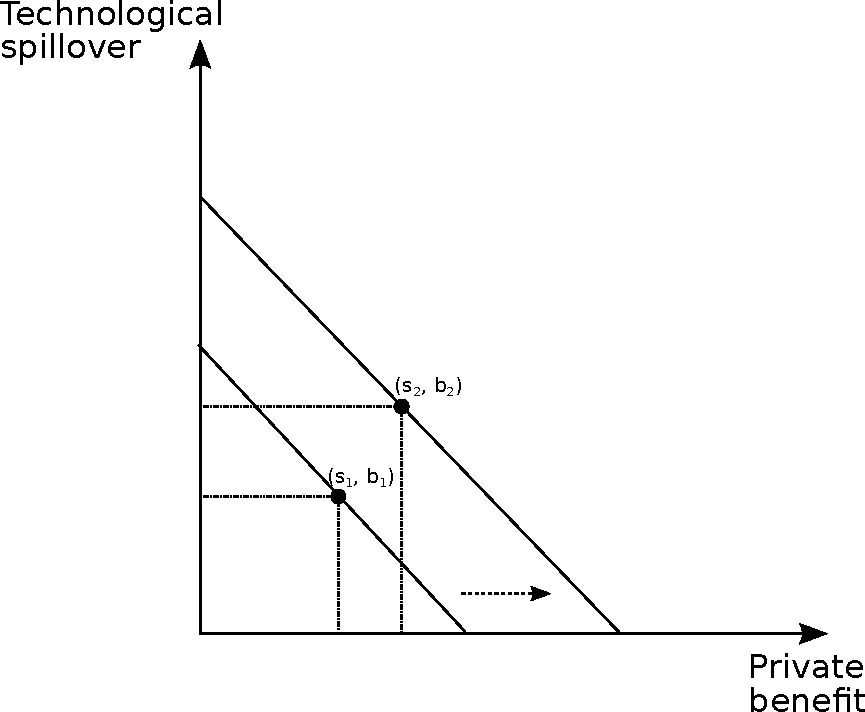
\includegraphics[width=0.75\textwidth, height=0.75\textheight,keepaspectratio]{../figure/budget_constraint}
    \caption{When an official has more endowment, his budget constraint shifts from left to right. He is now able to afford the $(b_2, s_2)$ bundle, with $b_2 > b_1$ and $s_2 > s_1$.}
    \label{fig:budget_constraint}
\end{figure}

\subsection{Parameter 2: The prices of spillover and private benefits determine the intercept and the slope of the budget constraint}
\label{sec:theory_budget_constraint_slope_and_intercept}

Given a fixed amount of the firm's profit to be shared with the official, the two intercepts of the budget constraint are determined by the ``price'' of the two goods, i.e. how easily the official can obtain technological spillover and private benefits from the foreign firm. If a good becomes harder to extract, the official can afford less of it and the corresponding intercept shifts inward (\Cref{fig:relative_price}). Alternatively, we can think of the slope of the budget constraint as the relative price of the two goods.

Substantively, the ``price'' of technological spillover depends on both the nature of the sector as well as the absorptive capacity of the local economy, which I define as the presence of domestic firms that are able to absorb technology from foreign firms.\footnote{I define \textit{domestic/private firms} as firms with over 50\% ownership belonging to private domestic individuals, companies, or organizations} Consider two channels through which technological spillover flows. First, domestic firms enter the supply chain of foreign firms, improving their productivity by imitating the higher production standards or management techniques of foreign firms. For this to happen, it is necessary to have a wealth of domestic firms that are technologically capable to enter the supply chain. The feasibility of such outsourcing is also sector-specific, e.g. whether the production process is divisible into units, or whether the technology has matured enough for subcontracting. Second, local employees working for foreign firms may learn from their experience and bring back knowledge when they move to private firms. For this to happen, domestic firms must also be technically advanced enough to make use of and compete for this high quality labor from the foreign sector.

The ``price'' of private benefit substantively means how easily the government officials can extract these benefits from the foreign firms. One example of such parameter is the origin of the foreign firm. Firms that come from countries where corruption is more common or accepted would be more adept at providing private benefits to official. In contrast, firms from countries that have signed onto the OECD anti-bribery convention could be more hesitant to bribe given the punishment that they may face from their home governments.

Changing prices of the two goods will move the intercept of the budget constraint and, holding the indifference curve constant, have implications for the mix of two goods that the official chooses.

\begin{figure}[!ht]
	\centering
    
\includegraphics[width=\textwidth, height=\textheight,keepaspectratio]{../figure/absorptive_capacity}
    \caption{In the left panel, the intercept for private benefits moves from right to left as its price increases. Similarly, in the right panel, as it becomes more difficult to extract spillover from foreign firms, the intercept moves down.}
    \label{fig:relative_price}
\end{figure}

\subsection{Parameter 3: The official's time horizon determines the shape of his indifference curve}
\label{sec:theory_indifference_curve}

The official has a convex indifference curve, implying a decreasing marginal utility to both spillover and private benefits. This assumption is standard and makes intuitive sense. As the official accumulates more private benefits, there are fewer things worth spending on as his consumption is satiated and produces less utility. Similarly, when more spillover happens, the lack of technological upgrading becomes less of a bottleneck to the economy. Thus, voters (or the official's higher-ups) become less concerned with the issue and it brings fewer electoral (or career) benefits.

The shape of the indifference curve denotes the relative weight the official assigns to the two goods, spillover and private benefits. When the curve is steep, the official is willing to trade a lot of spillover for a small increase in private benefits. Vice versa, a flatter curve indicates that the official values spillover more (\Cref{fig:indifference_curve}).

Politically, the steepness of the indifference curve depends on the time horizon of the official. This is because technological spillover takes time to materialize and to increase economic growth. In contrast, private benefits bring immediate utility. Therefore, the longer the official's time horizon, the more heavily does he value FDI spillover effect. For example, in \Cref{fig:indifference_curve}, the blue indifference curve is flatter and signifies more weight assigned to spillover. In that case, the official chooses a bundle that has more spillover and fewer private benefits (i.e. $s_1 > s_2$ and $b_1 < b_2$). Political factors that influence the official's time horizon may include term limit, the stability of the autocratic regime, or the degree of institutionalization of the party in power. 

\begin{figure}[!ht]
	\centering
    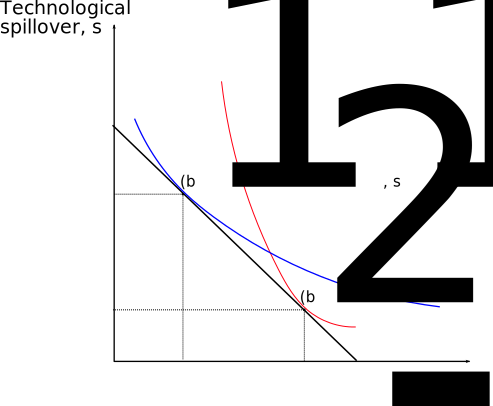
\includegraphics[width=0.75\textwidth, height=0.75\textheight,keepaspectratio]{../figure/indifference_curve}
    \caption{The blue indifference curve shows that the longer the official's time horizon, the flatter his indifference curve, and he will choose more spillover and fewer private benefits.}
    \label{fig:indifference_curve}
\end{figure}

\subsection{Literature on corruption and FDI}
\label{sec:theory_literature_review}

Regarding private benefits for the officials, I focus on corruption, i.e. bribe and informal fees, given the ubiquity of the practice in developing markets and wealth of data collected on this issue from cross-national business surveys. 

The majority of literature on the relationship between corruption and FDI focuses on showing that a high level of corruption deters FDI \citep{Wei2000, Hakkala2008, Al-Sadig2009}. A smaller literature examines the behaviors of foreign firms that choose to invest in a highly corrupt environment. It argues that foreign firms can help reduce corruption in host country via regulatory pressure effect, demonstration effect, and professionalization effect \citep{Kwok2006}; or via competing away the rents of the domestic firms and reducing the supply of bribes \citep{Sandholtz2003}. In these works, corruption between the host government and the foreign firm has been conceptualized as \textit{predatory}.

My research offers a new perspective, showing how corruption between government officials and foreign firms can be \textit{symbiotic}, with foreign firms getting exclusive access to resources, turning them into profits, and sharing the value added with the officials. Such symbiotic corruption between the government and foreign firm can be the key to explain the puzzle why governments may want to attract a lot of FDI despite the lack of developmental impact. (Corrupt) institutions matter, but not only to \textit{how much} FDI a country can attract as the literature has studied, but also \textit{which kind}.